\documentclass{article}

\usepackage[T1]{fontenc}
\usepackage{graphicx}
\usepackage{fancyhdr}
\pagestyle{fancy}
\fancyhf{}
\lhead{Version 1.3.1}
\rhead{Elliot Oram}
\rfoot{\thepage}


\title{Video Processor Class Diagram}
\author{elo9@aber.ac.uk}

\begin{document}

\maketitle
\tableofcontents

\newpage

\section{Video Processor Class Diagram}
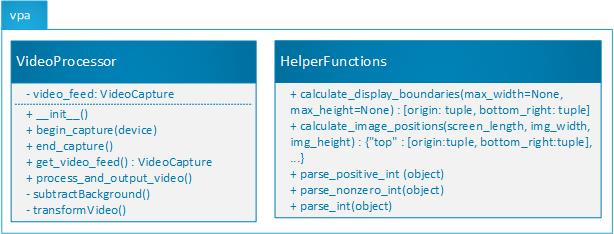
\includegraphics[width=\textwidth]{VideoProcessorClassDiagramImage}


\section{Description of Class Diagram}
The vpa (Video Processor Application) package contains two modules. The first, the \textbf{VideoProcessor} module, contains the \textbf{VideoProcessor} class which is the core of the system that will handle video capture and display. The second module will contain helper functions for the \textbf{VideoProcessor} class that do not require access to the class variables.

\subsection{VideoProcessor}
\subsubsection{Variables}
\begin{itemize}

	\item \textbf{video\_feed}: The video\_feed variable is of type VideoCapture. This class type holds a video stream and can be imported from OpenCV. To maximise the performance of the system the video object will be a global to the class object to avoid passing into and out of functions. However for test access there will be a get method for the video\_feed.
\end{itemize}

\subsubsection{Functions}

\begin{itemize}
	\item \textbf{\_\_init\_\_}: Python constructor for initialising the video\_feed object to None.
	
	\item \textbf{begin\_capture}: Function to start the video\_feed with specified device. This function takes an integer (referring to the device number to use - 0 is default) and sets the video\_feed to capture the video from that device. The function has a check to ensure that the parameter is an integer and raises a ValueError is it is not.
	
	\item \textbf{end\_capture}: Function to release the camera feed handle and set the video\_feed variable to None.
	
	\item \textbf{get\_video\_feed}: returns the video\_feed object.   

	\item \textbf{process\_and\_output\_video}: The output\_video function will add  4 copies of the video\_feed to a window in the correct locations. This function will also handle calls to subtract\_background and rotate\_image.

	\item \textbf{subtractBackground}: The subtractBackground function will be used to ensure that only the Actor is shown in the video feed and the background is removed (set to black (RGB(0,0,0)). Based on research stated in the Outline Project Specification, This will use simple background subtraction or moving average background subtraction. Spike solutions will be carried out during the creation of the prototype to assess if the image processing machine is capable of more complex background subtraction techniques. Furthermore, it will test if simple background subtraction techniques produce the required effect.

	\item \textbf{transformVideo}: The transformVideo function will duplicate the video feed into 4 identical. The feeds are rotated by 90 from one another around the centre of the display monitor.This is the format that is expected for the pyramid to produce holograms.
\end{itemize}


\subsection{HelperFunctions}
\subsubsection{Functions}

\begin{itemize}
	\item \textbf{calculate\_displa\_boundaries}: This function take the specified maximum width and height of the display area and creates the largest possible square that will fit. The function then returns the origin and bottom right co-ordinates of the square that will act as the maximum boundaries of the output window. If no values are provided for this function, the screen resolution is used instead.
	
	\item \textbf{calculate\_image\_positions}: Calculates the co\-ordinates that each image (video frame) should be placed in. The images should be in the top\-middle, bottom\-middle, left\-middle and right\-middle of the screen. The screen length (one require one value for this as the display area is square), image width and image height are parameters of the function. The function will calculate to co-ordinates by finding using half the screen length + or - half the height or width of the image. The function will return a map of lists of tuples containing the co-ordinates. The map will be structured such that: \\
	\{"position" : [origin tuple, bottom right tuple],\\... \} \\
	An example of this is: \\
	\{"top" : [(100,0), (200,50)],\\... \}

	\item \textbf{parse\_int}: Takes an object, python variable, and raises an error if it is not a integer. 	
	
	\item \textbf{parse\_positive\_int}: Takes an object, python variable, and raises an error if it is not a positive integer

	\item \textbf{parse\_nonzero\_int}: Takes an object, python variable, and raises an error if it a zero. 

\end{itemize}




\end{document}